
% JuliaCon proceedings template
\documentclass{juliacon}
\usepackage[ruled,vlined]{algorithm2e}
\setcounter{page}{1}

\keywords{landscape ecology , computational ecology,  julia programming language}

\makeatletter
\newcommand{\removelatexerror}{\let\@latex@error\@gobble}
\makeatother

\begin{document}

% **************GENERATED FILE, DO NOT EDIT**************

%\title{}

%\author[1]{}
%\author[2]{Kimberly Hall}
%\author[3]{Viral B. Shah}
%\author[1]{Alan Edelman}
%\affil[1]{Massachusetts Institute of Technology}
%\affil[2]{The Nature Conservancy}
%\affil[3]{Julia Computing Inc.}

%\keywords{landscape ecology , computational ecology,  julia programming language}


\maketitle

\begin{abstract}
Connectivity across landscapes influences a wide range of conservation-relevant ecological processes, including species movements, gene flow, and the spread of wildfire, pests, and diseases. The computational demands of the next generation of connectivity models and the availability of increasingly fine grained remote sensing data drive the need for faster software for connectivity modelling. To address this, we upgraded the widely-used Circuitscape connectivity package to the Julia programming language. The Julia package, Circuitscape.jl, can solve much larger problems up to an order of magnitude faster, with improved solvers and parallel computing features. We demonstrate scaling up to problems of 437 million grid cells, with speedups of up to 1800\% over the previous version. These improvements increase the pace of interaction between scientists and key stakeholders, facilitating faster policy decisions. 

\end{abstract}

\section{Introduction}
Connectivity models provide important insights into ecological processes that involve variation in movement or flow patterns across heterogeneous environments \cite{crooks2006}. In applied conservation, connectivity maps are incorporated into a wide range of resource evaluations and risk assessments. They inform decisions on how to sustain population dynamics and genetic diversity in plant and animal populations \cite{kareiva1995connecting}, how to most effectively prevent infectious disease spread or reduce risks from wildfire \cite{gray2016applying}, and choices of where to invest in land protection or restoration to help support species range shifts under a changing climate \cite{heller2009biodiversity, littlefield2017connecting, keeley2017habitat}.  

A common requirement for modeling connectivity is a gridded depiction of the landscape in which values for each cell represent some relative value of “resistance” to movement. These resistance grids are developed through several different methods, often involving iterative processes for categorizing resistance weights for different types of barriers based on expert opinion and information on species’ life histories and movement behaviors \cite{spear2010use, zeller2012estimating}. This grid can then be abstracted as a graph \cite{urban2001landscape}, providing a way to quantify ecological distance measures via graph-theoretic metrics. 

The range of mathematical approaches and software tools used for modeling connectivity reflect differences in theoretical approaches, and in the underlying assumptions about how movement proceeds. The classical isolation by distance model (IBD) posits that the least cost distance across the landscape graph acts as a good proxy for ecological distance \cite{wright1943isolation}.  Tools based on this approach typically identify a single “best” route between focal locations, an important result, but one that is highly dependent upon the choice of start and end points. It also has limited application if one’s goal is to compare potential options for restoration or protection across a landscape with multiple habitat patches and pathways.  As reviewed in \cite{dickson2019circuit}, from 2006-08, three seminal papers by the late Brad McRae built upon earlier work by \cite{doyle1984random} demonstrate that isolation by resistance (IBR)\cite{mcrae2006isolation} can provide an effective tool for considering connectivity potential across landscapes. IBR operationalizes the potential for genes and individuals to follow “random walks” across multiple pathways in the same way that electrical current flows across multiple resistors. These insights and McRae’s interest in informing conservation applications inspired the Circuitscape software package \cite{mcrae2008using}, which calculates effective resistance and “current flow,” a measure of net movement probability, across heterogeneous landscapes \cite{dickson2019circuit}.  This approach has evolved into a very flexible set of tools that allow users to vary the resistance grid and identification of what can be connected, enabling modelers to address a wide range of questions related to structural (ability of a landscape to support movement) and functional (modeling that is tailored to species-specific traits and behaviour) connectivity.  
Over the past decade Circuitscape has emerged as the most cited landscape connectivity tool in the world \cite{dickson2019circuit}. In the last year alone, Circuitscape has been cited 129 times, and in the past three years, 480 times. Dickson et al. (2019) reviews 277 applications of the software, in fields ranging from gene flow and animal movement to fire, water, and disease spread, and also describes how outputs are being used to inform conservation decisions. 


\begin{figure*}
    \centering
    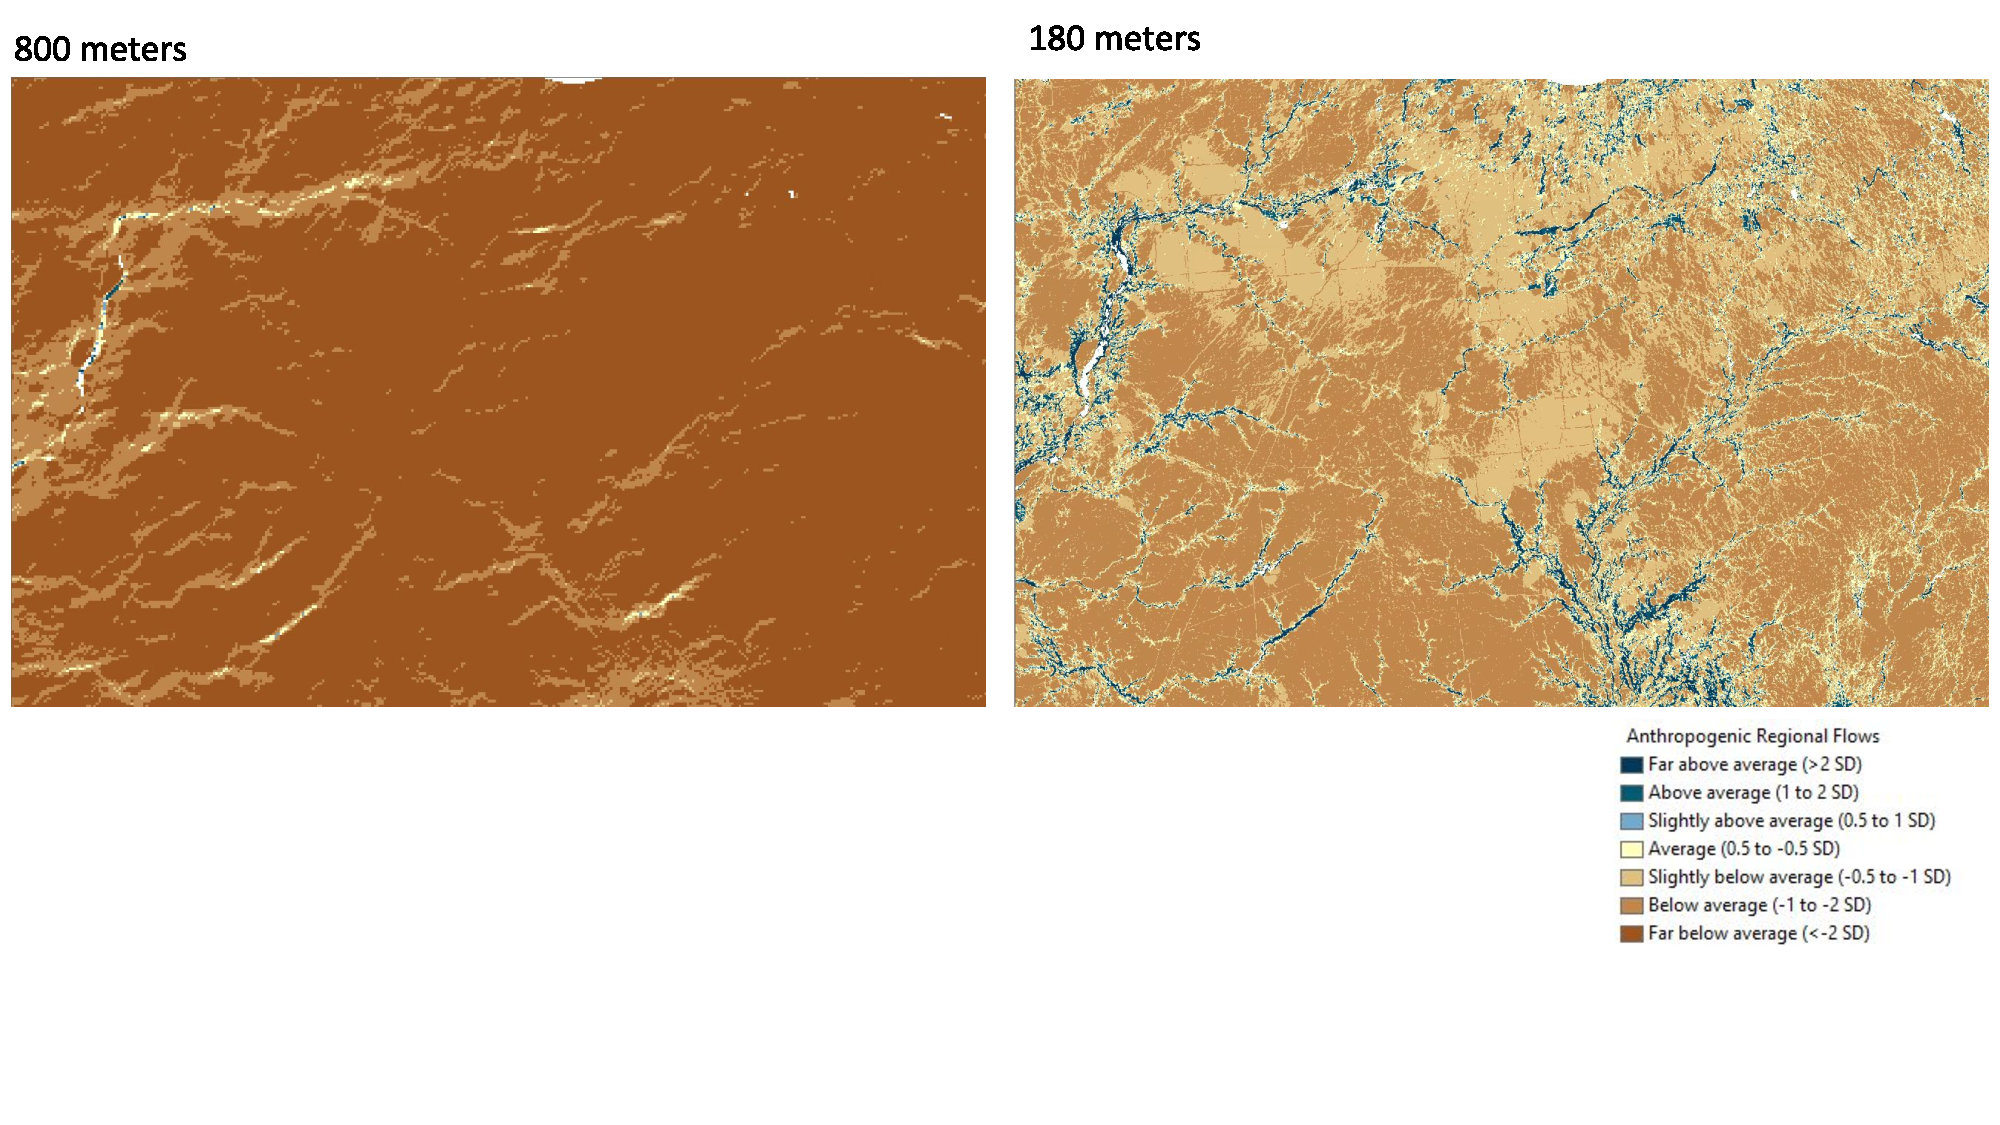
\includegraphics[width=\textwidth]{res.pdf}
    \caption{\textbf{An illustration of the impact of coarsening the resistance grid to address computational limitations.}  For this agricultural area along the border of Illinois and Indiana, USA, we show current flow derived from a resistance grid coarsened to 900m (left), compared to a higher-resolution map (180m cells, right).  Both resistance grids were derived from the 2011 NLCD (30m), and run with a “wall-to-wall” application of Circuitscape to evaluate landscape structural connectivity.  All “natural” terrestrial land cover types in the NLCD were assigned low resistance values, with pasture, roads, row crops, etc., assigned higher resistances. The 900m resolution map misses many narrow bands of natural land cover with high current flow (dark blue) indicating high connectivity value along streams and rivers. Analyses and maps by Melissa Clark, to support work in \cite{baldwin2018future}. 
}
    \label{fig:my_label}
\end{figure*}



\section{Circuitscape in Julia}
\label{sec:documentclass}
%
The goal of increasing the computational power of Circuitscape has been addressed multiple times by developers Brad McRae and Viral Shah.  McRae’s first version was written in Java, before being ported to MATLAB, to improve ease of development. Then, in collaboration with Tanmay Mohapatra, it was translated to Python for flexible scripting, platform independence and release under an open source license. This package makes heavy use of the numpy \cite{van2011numpy}, scipy \cite{jones2014scipy} and pyamg \cite{bell2015pyamg} numerical libraries and solves problems of up to tens of millions of nodes, but connectivity analysis on increasingly finer resolution datasets, typically hundreds of millions of nodes, and dozens of focal node pairs, a workload size well beyond its capacity. Circuitscape needed to be upgraded to support the newer demands of the user community. 

To address these demands, McRae and Shah collaborated on  a project called GFLOW \cite{leonard2017gflow}, a software tool for conducting circuit-theory based analyses on supercomputers. Written in the C programmming language and making use of solver libraries such as PetSc \cite{balay2004petsc} and BoomerAMG \cite{yang2002boomeramg}, GFLOW yields state of the art performance on large clusters and supercomputers. However, this performance comes at the cost of accessibility (does not work on the Windows operating system), composability (ability to integrate with other software libraries) as well as a tangible difficulty in shipping binaries because of their complicated build processes. For many practitioners and researchers, these constraints are a key barrier.

As the maintainers of Circuitscape, we saw the need for an open-source implementation that is easy to maintain, is high performance, is accessible to our user base and works well on every platform. We used the Julia programming language \cite{bezanson2017julia} to achieve this. Julia is an open source dynamic programming language that combines the readability of scripting languages such as R or Python, with the performance of a statically compiled language such as C or Fortran. With relatively little development effort via a straight reimplementation of the algorithm, Julia allowed us to not only significantly improve the package's computational capacity, but provide new user-facing features for free. For example, Julia's first class sparse matrix library and factorization support allowed us to support multiple solvers. Its modern Just in Time (JIT) compiler enables programmers to write generic code, then generate specialized code for desired precision, index types and hardware platform. This makes maintenance of the code base simple. Our upgrade, "Circuitscape.jl", is a registered Julia package and is already being used by the community to solve the next generation of connectivity problems.  

The rest of this paper is organized as follows: we present an overview of the algorithm in Section 3, followed by a description of the numerical methods and software packages in Section 4. Section 5 then briefly describes the new features introduced in the upgrade and present benchmarks both on synthetic problems and real user data. We conclude with a discussion on how speed improvements enable increased collaboration between computer scientists and ecologists, and improved collaboration between ecologists, conservation managers and other stakeholders. 

\section{The Algorithm}
\begin{figure}
\removelatexerror
\centering
\begin{algorithm}[H]
\SetAlgoLined
\LinesNumbered
\KwResult{Current (probability) maps $C$, nodal voltages $V$, pairwise resistances}
 Read input raster grid \;
 Read focal nodes \;
Construct undirected, weighted graph connecting neighboring cells\;
Compute graph Laplacian $G$ \;
\For{all pairs of focal nodes}{
    Set up $I$\;
    Solve linear system $GV = I$ \;
    Compute effective resistance $r$\;
    Write nodal voltages $V$ to disk\;
    Compute nodal currents from $I$ and write current map C to disk\
}

 \caption{Circuitscape - Pairwise Mode }
\label{alg1}
\end{algorithm}
\end{figure}

\begin{figure*}
    \centering
    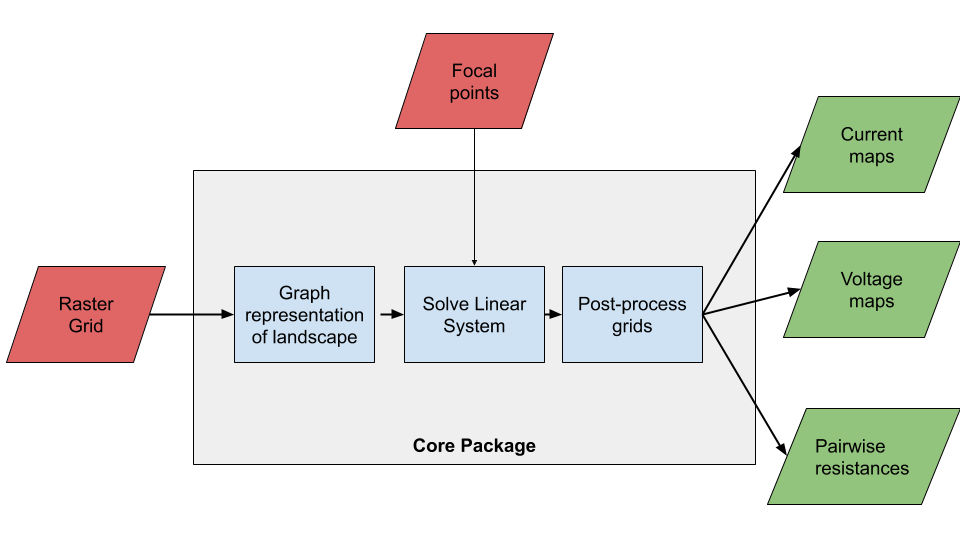
\includegraphics[width=0.5\textwidth]{flow.png}
    \caption{\textbf{Stages of computation and inputs/outputs}. The input raster grid to is usually assembled and produced using a GIS software package, and the output current maps are often exported to a GIS software package for postprocessing.}
    \label{fig:flow}
\end{figure*}

Circuitscape takes as input a raster grid, and a list of points (referred to as focal nodes) that are potential starting and ending points for animal movement. The raster grid is a spatial discretization of a heterogeneous landscape where each cell is assigned a value. Each value represents varying qualities of habitat, dispersal routes, or movement barriers. These “resistance” values are often problem specific, and either empirically derived based on movement or genetic data - or derived via expert opinion. This grid can then be represented as a graph, with nodes representing grid cells and edge weights proportional to the movement probabilities or number of migrants exchanged. Focal nodes represent points on the landscape of interest to the practitioner. These include habitat patches, protected areas, or populations to connect. These can be specified either through a raster grid with numerical labels for each focal point, or a text file with a list of coordinates. Once the graph is constructed, we then compute its Laplacian, which is an alternate representation of the landscape. We then solve for Ohm’s law using the computed graph Laplacian as the conductance matrix and the node locations of the focal points as current sources and sinks. For example, in raster-pairwise mode (described in Algorithm \ref{alg1}), Circuitscape loops through each possible source-sink pair and sets up a linear system per pair. On solving each system, we obtain a list of nodal voltages, which are then used to compute branch currents, that represent movement probabilities along branches of the graph. The ecological significance of these various quantities is summarized in related works \cite{mcrae2008using}. The branch currents are then accumulated on each node as nodal currents, which are then written to disk as a raster ASCII grid, for easy import into a geographic information system (GIS). This workflow has been summarized in Figure \ref{fig:flow}. 


\section{Numerical Methods}
The vast majority of the computation in Circuitscape is applying Ohm’s law and Kirchoff’s law over very large resistance grids, and solving a large sparse linear system: 
$$
GV = I
$$
where $G$ is the graph Laplacian representation of the landscape stored as a large sparse matrix, $I$ are the current sources, and $V$ are the nodal voltages. We provide two solver options to the user: the choleksy factorization and a preconditioned iterative method. The Cholesky factorization \cite{higham2009cholesky} is efficient for applications with smaller study areas and a large number of focal nodes. The sparse matrix is factored once and the solution to multiple pairs is computed via back substitution. Since the cost for backsubstitution is polynomially smaller than the cost of factorization, problems with a large number of focal pairs scale efficiently. The solver that scales to large problems is a preconditioned conjugate gradient (PCG) \cite{trefethen1997numerical}, with an algebraic multigrid preconditioner (AMG) \cite{vanvek1996algebraic}. We leverage Julia implementations of these methods from open source packages IterativeSolvers.jl \cite{iterativesolversjl} and AlgebraicMultigrid.jl \cite{amgjl}.

\subsection{Preconditioner Implementation}
Multigrid preconditioners are often used in problems solved across large spatial domains. In general, they take the original grid and generate a hierarchy of coarser grids, via predefined or algebraically derived restriction and interpolation operators. Large problems are solved by restricting quantities down to the coarsest level, obtaining a fast solution, and then interpolating the solution back to the original size. This procedure is often referred to as a “V” cycle. The efficacy of a good multigrid preconditioner is to with obtaining good restriction and interpolation operators. Usually, these operators are derived from the structure of the underlying problem. However, one can also estimate these operators algebraically, from the numerical values at each grid cell. This procedure is often referred to as Algebraic Multigrid (AMG). There are several variants of AMG, which are summarized in \cite{stuben2001review}. We use a variant called the Smoothed Aggregation AMG, which is known to work well for solving matrices generated by elliptic partial differential equations, such as Laplace’s equation. Laplacian matrices are structurally identical to the Laplacian of planar graphs that are generated in Circuitscape.


\section{New Features}

\subsection{New Solver Mode}

Circuitscape now supports a new solver based on the Cholesky factorization of the graph Laplacian representation of the landscape. We use the SuperNodal sparse cholesky factorization implemented in the CHOLMOD library \cite{chen2008algorithm}. The Julia programming language has first class sparse matrix library and matrix factorization support, which makes it easy to use this solver with a single function call. This solver mode also enables new approaches such as dividing the landscape into tiles to process independently \cite{pelletier2014applying} , and moving window analyses across the landscape \cite{mcrae2016conserving}. Both of these approaches produce fine scale and localized results. The obvious limitation of this solver, as with most sparse direct solvers, is that it works very well for relatively small matrices and runs out of memory for larger ones. This exponential growth in memory is a by-product of the factorization itself, as factors are often less sparse than the original matrix. 


\subsection{Generic Programming}

Julia supports the development of generic code while relying on the compiler to generate specialized code for different platforms and precision. Generic programs are powerful tools for our users, and can be made to adapt to their requirements. For example, the python package had a 32-bit integer type for indexing matrices hardcoded throughout the package, which limited the size of the computation the package ran. This led to crashes when running simulations for hundreds of millions of nodes. One such dataset studying the Mojave desert tortoise \cite{gray2019} used a resistance surface of 437 million pixels. This crashed the old version of Circuitscape, while the upgrade ran smoothly to completion. Circuitscape.jl defaults to a 32-bit integer type for cache efficiency, but provide users with a runtime flag to switch to 64-bit integer to index sparse matrices on the order of hundreds of millions. Since our Julia code was written generically, this feature came for free without any additional programming effort. Upgrading the python package to support this feature would require significant effort. 

\subsection{Improved Parallel Computations}

%Circuitscape.jl introduces support for parallelism on the Windows operating system. This was not possible with the Python package.

Parallel computing in Circuitscape.jl is inherently faster because the preconditioner can be serialized as a byte stream and sent over the network to other processes. This is not possible in the python code, as the python multiprocessing module internally uses the package pickle to serialize objects, and pyamg objects, implemented in C++, are not “pickle-able” \cite{pydoc}. The ability to serialize native Julia objects significantly reduced the amount of effort to parallelize Circuitscape.
In addition to faster parallel processing, we also extend parallelism support for more problem types in Circuitscape. In the benchmarks section, we demonstrate speed improvements on a dataset using these new features. The Julia version also lets the user call Circuitscape itself in parallel. As users aim to run Circuitscape over entire countries or continents, landscapes are often divided into multiple tiles \cite{pelletier2014applying}. This feature allows users to process (a batch of) these tiles by running different Circuitscape problem instances on each tile in parallel. These parallel features work on all platforms: Linux, MacOS and Windows. 

\section{Benchmarks}

\subsection{Experimental Setup}
We conducted our experiments on an Intel(R) Xeon(R) Silver 4114 CPU @ 2.20GHz with 384 GB of RAM. We used Julia v1.1.0 and Circuitscape v5.5.0, and compared against Circuitscape v4.0.5 

\subsection{Standard Benchmarks}
We benchmarked Circuitscape on standard synthetic problems. These benchmarks represent the most commonly used configuration and mode (Raster Pairwise) but with different problem sizes. These datasets can be found at \url{https://github.com/Circuitscape/BigTests/}. The benchmark results are summarized in Figure \ref{fig:csbench}. 

\begin{figure*}
    \centering
    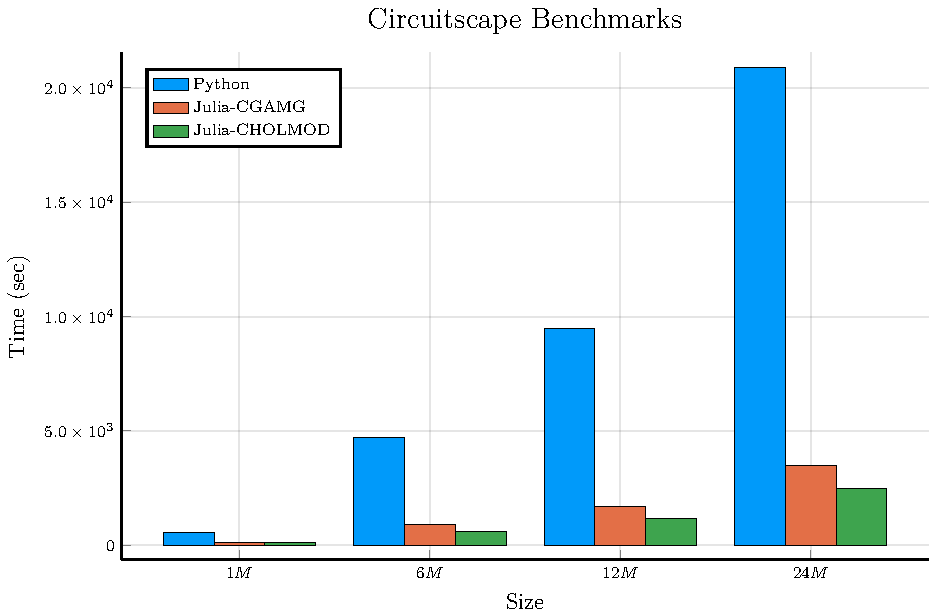
\includegraphics[width=0.5\textwidth]{bench.pdf}
    \caption{\textbf{Results on the standard Circuitscape benchmark suite (smaller is better)}. The red columns corresponds to Circuitscape.jl with the AMG solver, the green column coresponds to Circuitscape.jl with the Cholesky-based CHOLMOD solver, and the blue column correspnods to the old Python version of Circuitscape. Note that we benchmark only up to size 24M because at higher sizes the CHOLMOD solver runs out of memory and the Python version takes much, much longer. In summary, this chart demonstrates that Julia-CHOLMOD is the right choice for smaller problem sizes and Julia-CGAMG is the right choice for large problem sizes.}
    \label{fig:csbench}
\end{figure*}

\subsection{Benchmarks on Data from Existing Studies}

We ran the Python and Julia version of Circuitscape on a dataset used to model connectivity in the Sonoran desert \cite{drake2017using} (SONORAN). We used the all-to-one scenario \cite{mcrae2009circuitscape}, which models species migrating across the landscape from many different areas to one area. When the researcher used the old version of Circuitscape, this mode did not support parallelism, and the entire computation took over 2 days to run. Parallelism was trivial to support in the Julia version, which reduced execution time to less than 3 hours, resulting in a speedup of nearly 18x. We also benchmarked against a new range-wide model of connectivity for the endangered Mojave desert tortoise \cite{gray2019}(MOJAVE). We found that the Python version crashed, but the Julia package was able to scale effectively. The benchmark results are summarized in Figure \ref{table:bench}. 

\begin{figure*}
%\begin{table*}[]
\begin{tabular}{|l|l|l|l|l|}
\hline
\textbf{Benchmark} & \textbf{Size} & \textbf{Number of Solves} & \textbf{Time (Python)} & \textbf{Time (Julia)} \\ \hline
SONORAN            & 3339832       & 6002                      & 56.62 hrs              & 2.838 hrs             \\ \hline
MOJAVE             & 437 million   & 1                         & Crashed                & 3.385 hrs             \\ \hline
\end{tabular}
\centering
%\end{table*}
\caption{\textbf{Benchmarks on data from two conservation studies}. Two metrics determine the execution time of a Circuitscape run: the size of the problem and the number of linear system solves. Our package scales desirably in both directions. }
\label{table:bench}
\end{figure*}

\section{Discussion}

The growth in popularity of circuit theory to model ecological processes has to lead to widespread adoption of the Circuitscape software package. \cite{mcrae_shah_mohapatra_anantharaman}. The Circuitscape project has always evolved with the demands of the users and this upgrade to the Julia programming language seeks to drive the next generation of compute-intensive connectivity models - by shortening execution time from weeks to days and from days to hours. Users no longer have to coarsen their analysis due to computational limitations \cite{drake2017using}. Faster results often enhance stakeholder engagement, improve the feedback loop with policy makers and result in faster turnaround time for conservation decisions. Julia is already being used by ecologists to model ecological networks \cite{timothee_poisot_2018_1438428} and bioenergetic food webs \cite{delmas_eva_2019_2584373} and we see a strong role for it in other areas of computational ecology and conservation science. Its high level mathematical syntax is accessible to scientists while its speed allows them to simulate large, intricate models that capture complexity. We hope to see more ecologists and practitioners use and adopt Julia. 

% While connectivity tools typically focus in variation across space, questions related to temporal variability in connectivity, and simulations of how connectivity might change through habitat loss or restoration, would be of great interest as well.

\section{Conclusion}
We present an upgrade to the Circuitscape package, which will allow researchers to analyze ecological processes over large landscapes at fine resolutions. Our upgrade in the high performance Julia programming language presents upto a 1800\% improvement in computation time and the ability to solve problems on landscapes with hundreds of millions (and potentially billions) of grid cells. Julia’s sophisticated compiler allows for faster parallelism, generic programming and composability with other software packages. Circuitscape.jl is open source and is available at \url{https://github.com/Circuitscape/Circuitscape.jl} under the MIT license. Binaries are available on \url{https://circuitscape.org/downloads/}. It can also be installed using the Julia package manager by starting Julia, and entering \texttt{using Pkg; Pkg.add("Circuitscape")}. 

\section{Acknowledgement}
The work to update Circuitscape to the Julia computing language was funded through a grant from NASA’s Ecological Forecasting Program (16-ECO4CAST0018), and a grant from the Wilburforce Foundation.  The authors also wish to acknowledge the Wilburforce Foundation’s long-term investment in Circuitscape and related tools through several previous awards to Dr. Brad McRae.  We thank all of the Circuitsape users who have shared datasets, reported issues, and provided feedback on various versions of these tools, and look forward to continued collaboration with the user community. 

% **************GENERATED FILE, DO NOT EDIT**************

\bibliographystyle{juliacon}
\bibliography{ref.bib}

%\bibliography{ref}  %%% Remove comment to use the external .bib file (using bibtex).

\end{document}

% Inspired by the International Journal of Computer Applications template
